\section{树}
树是没有简单回路的连通无向图。一个无向图是树当且仅当在它的每对顶点之间都存在唯一简单通路。

\begin{itemize}
    \item 根树是指定一个顶点作为根并且每条边的方向都离开根的树。

    \item 有子女的顶点称为内点,根是内点。没有子女的顶点称为树叶。

    \item 若根树的每个内点都有不超过$m$个子女,则称它为$m$元树。若该树的每个内点都恰好有$m$个子女,则称它为正则$m$元树。$m=2$时的正则$m$元树称为二叉树。

    \item 在根树里顶点$v$的层是从根到该顶点的唯一通路的长度,根的曾定义为0。根树的高度就是顶点层数的最大值。

    \item 有序根树是把每个内点的子女们都排序的根树。
\end{itemize}

\subsubsection*{常用结论}
\begin{itemize}
    \item 带有$n$个顶点的树含有$n-1$条边。因为每一个不是根的顶点,都有唯一的一条向上的边,且这些边构成了树中所有的边。

    \item 带有$i$个内点的正则$m$元树含有$n = mi+1$个顶点。

    \item 一个正则$m$元树的顶点$n$、内点$i$、树叶$l$之间满足:
    \[i + l = n \] \[ n = mi + 1 \] \[ l = n - i = mi + 1 - i = (m-1)i + 1\]

    \item 在高度为$h$的$m$元树里至多有$m^k$个树叶。
    \item 若一个高度为$h$的$m$元树有$l$个树叶,则$h \ge \lceil \log_m l \rceil$。若这个$m$元树是正则的和平衡的,则$h = \lceil \log_m l \rceil$.
\end{itemize}

\subsubsection*{树的应用}
\begin{itemize}
    \item 二叉搜索树:基于一系列比较确定一个元素的位置(二分搜索),若树是平衡的,则确定一个项的位置或者添加一个项所需的比较次数不超过$\lceil \log (n+1) \rceil$.
    \item 决策树:通过一步一步的决策构建问题的解,从根到树叶的通路都是问题的可能解。可以使用决策树来确定排序算法的最坏情形复杂度等。
    \item 前缀码:使用不同长度的位串来编码字母,较短的位串用于编码频繁的字母,较长的位串用于编码不经常出现的字母。如赫夫曼编码:
    \begin{center}
        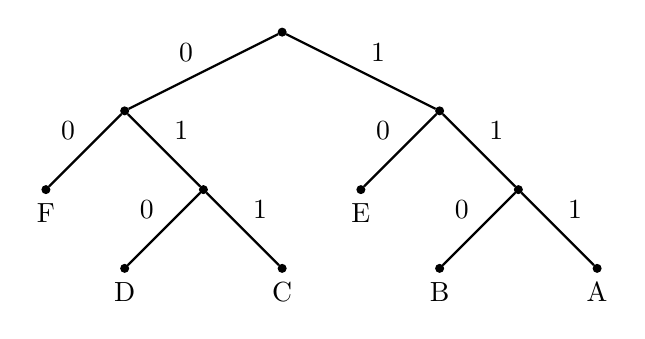
\begin{tikzpicture}
            [dot/.style={circle,inner sep=1pt,draw=black,fill=black},line/.style={thick}]
            \node[dot,label=below:A] (a) at (4,0) {};
            \node[dot,label=below:B] (b) at (2,0) {};
            \node[dot,label=below:C] (c) at (0,0) {};
            \node[dot,label=below:D] (d) at (-2,0) {};
            \node[dot] (ab) at (3,1) {}
                edge[line] node[auto] {1} (a)
                edge[line] node[auto,swap] {0} (b);
            \node[dot,label=below:E] (e) at (1,1) {};
            \node[dot] (cd) at (-1,1) {}
                edge[line] node[auto] {1} (c)
                edge[line] node[auto,swap] {0} (d);
            \node[dot,label=below:F] (f) at (-3,1) {};
            \node[dot] (abe) at (2,2) {}
                edge[line] node[auto] {1} (ab)
                edge[line] node[auto,swap] {0} (e);
            \node[dot] (cdf) at (-2,2) {}
                edge[line] node[auto] {1} (cd)
                edge[line] node[auto,swap] {0} (f);
            \node[dot] (all) at (0,3) {}
                edge[line] node[auto] {1} (abe)
                edge[line] node[auto,swap] {0} (cdf);
        \end{tikzpicture}
    \end{center}
    \item 博弈树:博弈树通常用于描述二人轮流的游戏,每个树叶表示游戏结局的一种。
    \begin{enumerate}
        \item 每个树叶为游戏结束时第一个玩家的分数;
        \item 偶数层顶点的值选择子女中的最大值,奇数层的值顶点选择子女中的最小值。因为第二个玩家的回合总是想让第一个玩家的分数降低。这种策略称为最小最大策略。若两个玩家都严格遵循最小最大策略,则可以计算哪位玩家获胜。
    \end{enumerate}
\end{itemize}

\subsection{遍历}
通用地址系统:用整数0标记根,然后用$1,2,3,\cdots,k$从左向右标记它的$k$个子女;对于一个已经标记为$A$的内点,从左向右依次标记它的$k$个子女为$A.1, A.2, \cdots, A.k$.

系统地访问有序根树的每个顶点的过程称为遍历算法。三个最常用的遍历算法是:前序遍历、中序遍历、后序遍历。

\begin{itemize}
    \item 前序遍历:设$T$是带根$r$的有序根树。若只包含$r$,则$r$是$T$的前序遍历。否则,假定$T_1,T_2,\cdots,T_k$是$r$的从左向右的子树,前序遍历首先访问$r$,再依次\uline{以前序来遍历}$T_1,T_2,\cdots,T_k$.
    \item 中序遍历:设$T$是带根$r$的有序根树。若只包含$r$,则$r$是$T$的中序遍历。否则,假定$T_1,T_2,\cdots,T_k$是$r$的从左向右的子树,中序遍历首先\uline{以中序来遍历}$T_1$,再访问$r$,最后依次\uline{以中序来遍历}$T_2,\cdots,T_k$.
    \item 后序遍历:设$T$是带根$r$的有序根树。若只包含$r$,则$r$是$T$的后序遍历。否则,假定$T_1,T_2,\cdots,T_k$是$r$的从左向右的子树,后序遍历首先依次\uline{以后序来遍历}$T_1,T_2,\cdots,T_k$,再访问$r$.
\end{itemize}

\subsubsection*{表达式的前缀、中缀和后缀记法}
对表达式的二叉树的前序、中序和后序遍历形成其前缀、中缀和后缀记法。前缀形式也称作波兰记法。

\subsection{生成树和最小生成树}

\subsubsection*{生成树}
设$G$是简单图,$G$的生成树是包含$G$的每个顶点的$G$的子图。再$G$的基础上删去一些边来形成树。

简单图是连通的当且仅当它具有生成树。

构建生成树的算法分为深度优先搜索算法和宽度优先搜索算法。以下图为例:
\begin{center}
    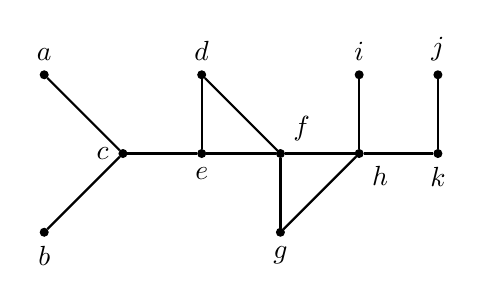
\begin{tikzpicture}
        [dot/.style={circle,inner sep=1pt,draw=black,fill=black},
        line/.style={thick}]
        \node[dot,label=above:$a$] (a) at (-3,1) {};
        \node[dot,label=below:$b$] (b) at (-3,-1) {};
        \node[dot,label=left:$c$] (c) at (-2,0) {}
            edge[line] (a)
            edge[line] (b);
        \node[dot,label=above:$d$] (d) at (-1,1) {};
        \node[dot,label=below:$e$] (e) at (-1,0) {}
            edge[line] (c)
            edge[line] (d);
        \node[dot,label=above right:$f$] (f) at (0,0) {}
            edge[line] (d)
            edge[line] (e);
        \node[dot,label=below:$g$] (g) at (0,-1) {}
            edge[line] (f);
        \node[dot,label=below right:$h$] (h) at (1,0) {}
            edge[line] (f)
            edge[line] (g);
        \node[dot,label=above:$i$] (i) at (1,1) {}
            edge[line] (h);
        \node[dot,label=above:$j$] (j) at (2,1) {};
        \node[dot,label=below:$k$] (k) at (2,0) {}
            edge[line] (h)
            edge[line] (j);
    \end{tikzpicture}
\end{center}

\subsubsection*{深度优先搜索}
以$f$为起点构建一条到一个树叶的通路,顶点不重复,如选择$f-g-h-k-j$做为起始的树。从最后的顶点回溯,不存在以$k$开始且含有不在树上的顶点的通路;然后回溯到$h$,存在以$h$开始且含有不在树上的顶点的通路$h-i$,将它添加到树上;依次向上回溯,可以构建出如下的树:
\begin{center}
    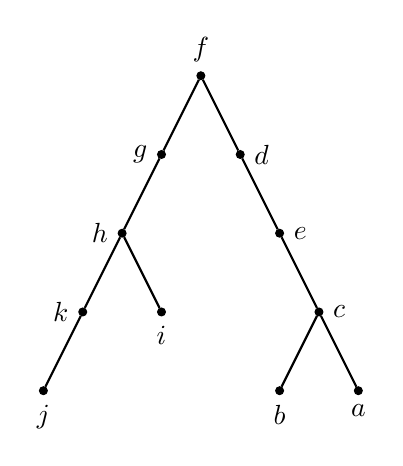
\begin{tikzpicture}
        [dot/.style={circle,inner sep=1pt, draw=black, fill=black},
        line/.style={thick}]
        \node[dot,label=below:$a$] (a) at (2,0) {};
        \node[dot,label=below:$b$] (b) at (1,0) {};
        \node[dot,label=below:$j$] (j) at (-2,0) {};
        \node[dot,label=right:$c$] (c) at (1.5,1) {}
            edge[line] (a)
            edge[line] (b);
        \node[dot,label=below:$i$] (i) at (-0.5,1) {};
        \node[dot,label=left:$k$] (k) at (-1.5,1) {}
            edge[line] (j);
        \node[dot,label=right:$e$] (e) at (1,2) {}
            edge[line] (c);
        \node[dot,label=left:$h$] (h) at (-1,2) {}
            edge[line] (k)
            edge[line] (i);
        \node[dot,label=right:$d$] (d) at (0.5,3) {}
            edge[line] (e);
        \node[dot,label=left:$g$] (g) at (-0.5,3) {}
            edge[line] (h);
        \node[dot,label=above:$f$] (f) at (0,4) {}
            edge[line] (d)
            edge[line] (g);
    \end{tikzpicture}
\end{center}

\subsubsection*{宽度优先搜索}
选取$f$为根,将与$f$相邻的所有的顶点作为$f$的子女,添加到1层上。然后将于1层上的顶点相邻且不在树上的顶点,作为对于的顶点的子女,添加到2层上。依次类推,可以构建出如下的树:

\begin{center}
    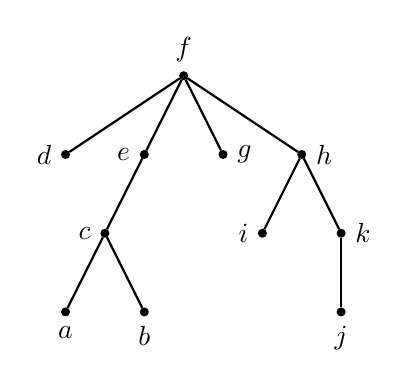
\begin{tikzpicture}
        [dot/.style={circle,inner sep=1pt, draw=black, fill=black},
        line/.style={thick}]
        \node[dot,label=below:$a$] (a) at (-1.5,0) {};
        \node[dot,label=below:$b$] (b) at (-0.5,0) {};
        \node[dot,label=below:$j$] (j) at (2,0) {};
        \node[dot,label=left:$c$] (c) at (-1,1) {}
            edge[line] (a)
            edge[line] (b);
        \node[dot,label=left:$i$] (i) at (1,1) {};
        \node[dot,label=right:$k$] (k) at (2,1) {}
            edge[line] (j);
        \node[dot,label=left:$d$] (d) at (-1.5,2) {};
        \node[dot,label=left:$e$] (e) at (-0.5,2) {}
            edge[line] (c);
        \node[dot,label=right:$g$] (g) at (0.5,2) {};
        \node[dot,label=right:$h$] (h) at (1.5,2) {}
            edge[line] (k)
            edge[line] (i);
        \node[dot,label=above:$f$] (f) at (0,3) {}
            edge[line] (d)
            edge[line] (e)
            edge[line] (g)
            edge[line] (h);
    \end{tikzpicture}
\end{center}

\subsubsection*{最小生成树}
连通带权图里的最小生成树是具有最小可能的边的权之和的生成树。

构建最小生成树可以使用普林算法和克鲁斯卡尔算法。
\begin{itemize}
    \item 普林算法:首先选择带最小权的边,把它放进生成树里。相继地向树里添加与已在树里的顶点相关联的、并且不与已在树里的边形成简单回路的权最小的边。当已经添加了$n-1$条边时停止。
    \item 克鲁斯卡尔算法:首先选择图中权最小的一条边,把它放进树里,相继地添加不与已在树里的边形成简单回路的权最小的边。当已经添加了$n-1$条边时停止。
\end{itemize}

\section{布尔代数}
\subsection{布尔代数的概念与表示}
\begin{itemize}
    \item 3种常用的布尔运算:补$\overline x$、和$x+y$、积$x \cdot y$对应NOT、OR、AND.

    \item 布尔函数:$y = f(x_1,x_2,\cdots,x_n)$,其中$x$称为布尔变元,$x_1,x_2,\cdots,x_n,y \in \{0,1\}$.
    \item 以$X$表示$x_1,x_2,\cdots,x_n$,有以下结论:
    \begin{itemize}
        \item $\overline F(X) = \overline{F(X)}$
        \item $(F+G)(X) = F(X) + G(X)$
        \item $(FG)(X) = F(X)G(X)$
    \end{itemize}

    \item 布尔恒等式:
    \begin{itemize}
        \item $\overline {\overline x} = x$
        \item $x+x = x,x \cdot x = x$
        \item $x+0 = x, x \cdot 1 = x$
        \item $x+1 = 1, x \cdot 0 = 0$
        \item $x+y = y+x, xy = yx$
        \item $x+(y+z) = (x+y)+z, x(yz) = (xy)z$
        \item $x + yz = (x+y)(x+z), x(y+z) = xy + xz$
        \item $\overline {(xy)} = \overline x + \overline y,\overline{(x+y)} = \overline x \overline y$
        \item $x + xy = x,x(x+y) = x$
        \item $x + \overline x = 1, x \overline x = 0$
    \end{itemize}
    恒等式中经常有两个式子同时出现,这种关系可以称为对偶。可以交换积与和,交换0与1,来获得一个式子相对偶的式子。

    \item 文字:布尔变元或者它的补称为文字。

    小项:$n$个文字的积。

    布尔表达式可以化简成多个小项的和,称为积之和展开式或析取范式。
\end{itemize}

\subsubsection*{电路最小化}
将一个布尔表达式化简成最简的积之和展开式。这时实现这样的逻辑所需的电路元件最少。

\begin{itemize}
    \item 卡诺图:适用于布尔变元较少的情况。以两个布尔变元为例:
    \begin{center}
        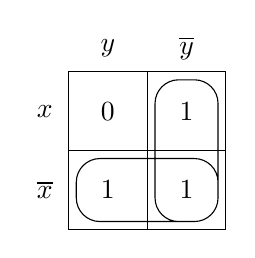
\begin{tikzpicture}
            \draw (-1,0) rectangle (0,1)
                (0,0) rectangle (1,1)
                (-1,-1) rectangle (0,0)
                (0,-1) rectangle (1,0);
            \node at (-0.5, 0.5) {0};
            \node at (0.5,0.5) {1};
            \node at (-0.5, -0.5) {1};
            \node at (0.5,-0.5) {1};
            \node at (-1.3,0.5) {$x$};
            \node at (-1.3,-0.5) {$\overline x$};
            \node at (-0.5,1.3) {$y$};
            \node at (0.5,1.3) {$\overline y$};
            \draw [rounded corners=3mm] (0.1,-0.9) rectangle (0.9,0.9)
                (-0.9,-0.9) rectangle (0.9,-0.1);
        \end{tikzpicture}
    \end{center}

    上图中圆角矩形横跨了$\overline x$的一行,此时表明$\overline x$必会发生,可以将圆角矩形中两个格子代表的元素合成一个$\overline x$。同理,另一个圆角矩形将两个格子合成$\overline y$,因此,这个图表示的是$x \overline y + \overline x y + \overline x \cdot \overline y = \overline x + \overline y$.

    \item 奎因-莫可拉斯基方法
    当布尔变元较多时,卡诺图的方法就不方便。可以使用奎因-莫克拉斯基方法。
    首先将$n$个变元构成的小项,用$n$位二进制位串表示,其中$x$用1表示,$\overline x$用0表示。
    然后根据串中1的个数将这些串分组,仅相差一位二进制的串可以合并,合并后的串中不同的那位二进制用'-'表示。
    只要能够合并就继续合并,直到不能合并为止。将合并的结果还原回小项,其中的'-'表示没有这一变元。
\end{itemize}

\section{计算模型}
\subsection{有限状态机}
\begin{itemize}
    \item 有限状态机:设$M = (S, I, O, f, g, s_0)$,其中$S$表示有限状态的集合,$I$表示输入字母表,每个字母代表一种输入,$O$表示输出字母表,每个字母代表一种输出。转移函数$f$输入一种状态和输入字母,就会产生一种状态。输出函数$g$输入一种状态和输入字母,就会产生一种输出字母。$s_0$表示初始状态。

    有限状态机可以使用状态表或者带有标号边的有向图来表示。

    设有限状态机$M$,当存在一个集合$L \subset I$且$L$中的所有元素作为$M$的输入时,$M$的输出均为1,称$M$能够识别(或接受)$L$.
    
    有限状态机可以分为米利机和摩尔机。米利机的输出与初始状态和输出都有关系,而摩尔机的输出只与初始状态有关系。
    
    \item 有限状态自动机:是一种没有输出的有限状态机。设$M = (S, I, f, s_0, F)$,其中$F$为终结状态。

    转移函数扩展:若$f(s, xy) = f(f(s,x),y)$,则称该状态机可以转移函数扩展。

    \item 非确定型有限状态自动机:设$M = (S, I, f, s_0, F)$,与有限状态自动机不同的是,转移函数给出的输出状态可能是多个状态中的一个。
    
    \item 更强大的机器:下推自动机、线性有界自动机、图灵机
\end{itemize}

\subsection{语言处理}
\begin{itemize}
    \item 词汇表$V^*$.
    \item 词汇表在一定的文法下产生的所有符串的集合记作$L(G)$.
    \item 克莱因闭包:设$A \subset V^*$,则$A$的克莱因闭包是$A$中的任意多个串的组合而形成发集合,记作$A^*$。
    \item 如果语言$L$可以由一个非确定型有限状态自动机识别,则它必定可以由一个确定型有限状态自动机识别。
    \item 正则集合:从空集、空串、单字符串开始,以任意顺序连接,并和克莱因闭包运算所得的。
    \item 克莱因定理:一个集合是正则的,当且仅当它可以由一个有限状态机识别。
    \item 一个集合可以由正则文法形成,当且仅当它是一个正则集合。
\end{itemize}


\subsection{计算复杂度、可计算性、可判定性}
\begin{itemize}
    \item 判定问题:是与不是的问题。

    可判定性:当存在一个算法来判断判定问题的某个解是否正确,则称这个问题是可判定的。

    \item \uline{停机问题}:停机问题是不解的判定问题,当给定图灵机$T$的编码及输入串$x$,没有图灵机能够判定该图灵机$T$最终是否会停机。

    \item 可计算性:如果一个函数可以被图灵机计算,则称这个函数是可计算的。

    \item P类问题:如果一个判定问题可以用确定型图灵机在多项式时间内求解,则这个问题是P类问题,即确定型多项式时间问题。

    NP类问题:如歌一个判定问题可以用非确定型图灵机在多形式时间内求解,则这个问题是NP类问题,即非确定型多项式时间问题。

    属于P类问题的是易处理的,不属于P类问题的是不易处理的。P$\subset$NP.
\end{itemize}